\documentclass[9pt]{report}

\usepackage{talk}
\usepackage{mathpazo}
\renewcommand{\baselinestretch}{1.05}
% \usepackage[export]{adjustbox}

\newcommand{\draw}[2]{#1^{(#2)}}
\newcommand{\displayfrac}[2]{{\displaystyle \frac{\displaystyle #1}{\displaystyle #2}}}
\newcommand{\simvar}[1]{#1^{\textrm{sim}}}
\newcommand{\simdraw}[2]{#1^{\textrm{sim}(#2)}}

\begin{document}
\sf%
\mbox{ }
\\[12pt]
\spc{\Large\bfseries \myemph{SARS-CoV-2 diagnostic testing:}}
\\[4pt]
\spc{\Large\bfseries \myemph{test site variation and time trends}}
\\[36pt]
\noindent
\spc{\bfseries \myemph{Bob Carpenter}}
\\[2pt]
\spc{Center for Computational Mathematics}
\\[2pt]
\spc{Flatiron Institute}
\vfill
\noindent
\spc{\small \myemph{@ Paris Diderot / INSERM}} \hfill

\includegraphics[height=24pt]{img/flatiron-logo.png}
\hfill

\includegraphics[height=24pt]{img/stan-logo.png}

\sld{SARS-CoV-2 test accuracy varies}

\begin{itemize}
\item by testing \myemph{site}
\item by \myemph{time} since infection
\item by \myemph{test type} (PCR vs. lateral flow)
\item and presumably by \myemph{variant} (alpha, delta, omicron, $\ldots$)
\end{itemize}

\sld{Sensitivity and specificity}
\begin{itemize}
\item \myemph{sensitivity} is accuracy on positive cases
\item \myemph{specificity} is accuracy on negative cases
\item if $Z_n$ is disease status for subject $n$ and $Y_n$ is test result,
  \begin{subitemize}
  \item $\textsf{sensitivity} = \textrm{Pr}[Y_n = 1 \mid Z_n = 1]$
  \item $\textsf{specificity} = \textrm{Pr}[Y_n = 0 \mid Z_n = 0]$
  \end{subitemize}
\end{itemize}

\sld{Diagnosis \& calibration}
\begin{itemize}
\item for \myemph{diagnostic testing},
  \begin{subitemize}
  \item test result $Y_n$ is \myemph{observed}, but
  \item disease status $Z_n$ is \myemph{latent}
  \end{subitemize}
\item for \myemph{calibration testing},
  \begin{subitemize}
  \item test result \myemph{and} disease status are \myemph{observed}
  \item \myemph{known negatives} use pre-Covid blood samples
  \item \myemph{known positives} are independently verified cases
  \end{subitemize}
\end{itemize}

\sld{Population prevalence}
\begin{itemize}
\item \myemph{prevalence} is proportion of population who are
  positive
\item we use $\pi \in [0, 1]$ for prevalence
\item \myemph{prevlaence varies} by the following (among other things!)
  \begin{subitemize}
  \item time 
  \item geo-location
  \item age
  \item sex
  \item socio-economic status
  \item ethnicity
  \item intervention
  \end{subitemize}
\end{itemize}
  
\sld{Inferential goals}
\begin{itemize}
\item we have three goals in modeling diagnostic tests
  \begin{subitemize}
  \item estimate \myemph{diagnostic accuracy}: $\textrm{Pr}[Y_n \mid Z_n])$
  \item estimate \myemph{population prevalence}: $p(\pi \mid Y, Z)$
  \item provide probabilistic \myemph{diagnostics}: $\textrm{Pr}[Y_n = 1 | Z_n]$
  \end{subitemize}
\end{itemize}

\sld{Bayesian modeling}
\begin{itemize}
\item Andrew Gelman says \myemph{Donald Rubin advises}:
  \begin{subitemize}
  \item model what we'd do if we \myemph{had all the data},
  \item then \myemph{turn the Bayesian crank} to infer unknowns
  \end{subitemize}
\item This allows us to design models without
  \begin{subitemize}
  \item worrying about the \myemph{details of inference}
  \item deciding a priori how to handle \myemph{``missing'' data}
  \end{subitemize}
\end{itemize}

\sld{Model basics for site variation}
\begin{itemize}
\item diagnostic tests known to \myemph{vary by test site}
\item we will build up to a model where
  \begin{subitemize}
  \item \myemph{likelihood}: sensitivity and specificity vary by site
    and individuals are \myemph{exchangeable}
  \item \myemph{prior}: hierarchical population model of site sensitivity and specificity
  \end{subitemize}
\item we will \myemph{observe}
  \begin{subitemize}
  \item \myemph{test site and result} for each individual
  \item \myemph{disease status} fo some individuals
  \end{subitemize}
\end{itemize}

\sld{Variable notation}
\begin{itemize}
  \item \myemph{parameters}
  \begin{subitemize}
  \item $\pi \in (0, 1)$: \myemph{prevalence} of infection in population
  \item $\theta_{k, 1}$: \myemph{sensitivity} at test site $k \in 1:K$
  \item $\theta_{k, 0}$: \myemph{specificity} at test site $k \in 1:K$
  \end{subitemize}
\item \myemph{data} (both observed and \myemph{``missing''}
  \begin{subitemize}
  \item $N$ total test \myemph{subjects}
  \item $y_n \in \{ 0, 1 \}$: \myemph{test result}
  \item $z_n \in \{ 0, 1 \}$: \myemph{disease status} of subject $n$
  \item $kk_n \in 1{:}K$: \myemph{site} for test $n$
  \item $y_n \in \{ 0, 1 \}$: \myemph{test result} for individual $n$
  \end{subitemize}
\end{itemize}

\sld{Start without site variation}
\begin{itemize}
\item start with simple model, then criticize and revise
  \begin{subitemize}
  \item baseline model from \myemph{Bendavid et al.} (2020)
    \end{subitemize}
\item assume sensitivty and specificity \myemph{do not vary} by
  site
\item two views on lack of variation
  \begin{subitemize}
  \item \myemph{choice of prior}: (e.g., $\theta_{i, k} = \theta_{i, k'}$), or
  \item \myemph{choice of likelihood}: one parameter each for sensitivity
    \& specificity
  \end{subitemize}
\end{itemize}

\sld{Simple non-varying model}

\begin{itemize}
\item let $\theta_1$ be \myemph{sensitivity} and $\theta_0$ \myemph{specificity}
\item uniform \myemph{priors} on probabilites
  \begin{subitemize}
  \item $\pi, \ \theta_1, \ \theta_0 \sim \textrm{uniform}(0, 1)$
  \item equivalently, standard logistic prior on log odds
  \end{subitemize}
\item \myemph{``complete'' data likelihood} for missing \& non-missing
  \begin{subitemize}
  \item $z_n \sim \textrm{bernoulli}(\pi)$
  \item $y_n \sim
    \begin{cases}
      \textrm{bernoulli}(\theta_1) & \textsf{if } z_n = 1
      \\
      \textrm{bernoulli}(1 - \theta_0) & \textrm{if } z_n = 0
    \end{cases}$
  \end{subitemize}
\item \myemph{calibration} cases have observed $z_n$
\end{itemize}

\sld{Data and fit for simple model}
\begin{subitemize}
\item \myemph{positive calibration} ($z_n = 1$): 103 / 122
\item \myemph{negative calibration} ($z_n = 0$) : 399 / 401
\item \myemph{missing disease status} ($z_n$ unknown): 50 / 3300
\end{subitemize}
\vspace*{-6pt}
\begin{center}
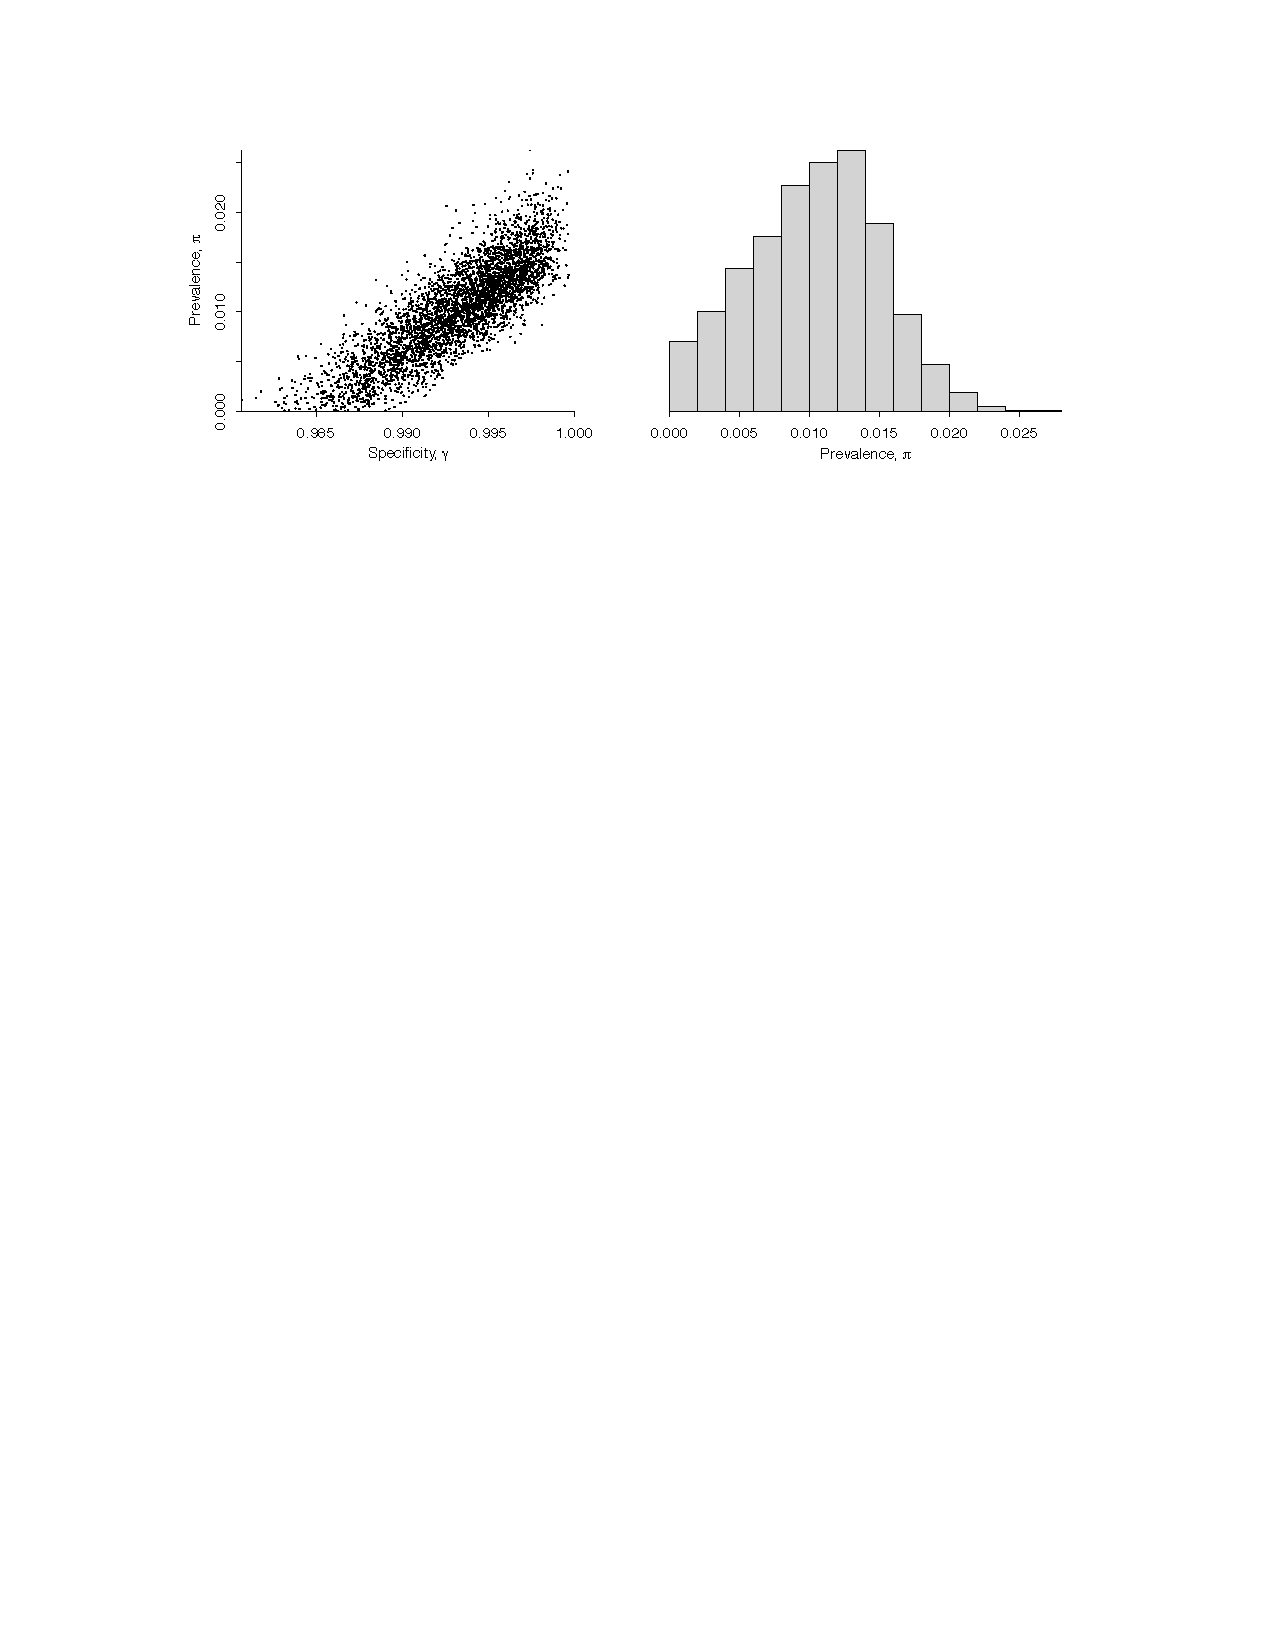
\includegraphics[width=0.9\textwidth]{img/simple-inf.pdf}
\end{center}
\vspace*{-8pt}
\begin{subitemize}
\item 95\% \myemph{shortest posterior interval} (0, 1.8\%) for $\pi$ \myemph{inconclusive}
\end{subitemize}

\sld{Hierarchical model}
\begin{itemize}
  \item \myemph{hierarchical priors} for sensitivity and specificity
\begin{subitemize}
\item \myemph{specificity}: $\textrm{logit}(\theta_{k, 0}) \sim \textrm{normal}(\mu_0, 
  \sigma_0)$
\item \myemph{sensitivity}: $\textrm{logit}(\theta_{k, 1}) \sim \textrm{normal}(\mu_1, 
  \sigma_1)$
\end{subitemize}
\item \myemph{hyperpriors} for hierarchical parameters
  \begin{subitemize}
  \item hyperprior mean: $\mu_0, \mu_1 \sim \textrm{normal}(2, 4)$
  \item hyperprior scale (specificity): $\sigma_0 \sim \textrm{normal}_+(0, \tau_0)$
  \item hyperprior scale (sensitivity): $\sigma_1 \sim
    \textrm{normal}_+(0, \tau_1)$
  \end{subitemize}
\item we evaluate \myemph{broad} and \myemph{weakly
    informative} priors
  \begin{subitemize}
  \item weakly informative set \myemph{expected scale} and \myemph{regularize}
  \end{subitemize}
\end{itemize}


\sld{Multivariate hierarchical model}
\begin{itemize}
  \item sensitivity and specificity are \myemph{correlated}
    \begin{subitemize}
    \item \myemph{positively} due to care taken by lab
    \item \myemph{negatively} based on decision threshold
    \end{subitemize}
  \item we'd like to impose a \myemph{multivariate prior}
  $$\begin{bmatrix} \theta_{0, k} & \theta_{1, k} \end{bmatrix}
  \sim \textrm{multi-normal}(\mu, \Omega)$$
  \vspace*{-12pt}
  \begin{subitemize}
    \item but no sites in our data have \myemph{positive {\slshape and}\ negative}
      calibration tests
    \end{subitemize}
\end{itemize}
  
\sld{Inferences from hierarchical model}
\vspace*{-12pt}
\begin{subitemize}
  \item site $k = 1$ has diagnostic tests with \myemph{unknown disease
      status}
    \vspace*{-4pt}
  \item yielding estimates for \myemph{population prevalence} and
    \vspace*{-4pt}
  \item estimates for \myemph{test accuracy} at a \myemph{site with no calibration data}
\end{subitemize}
\qquad 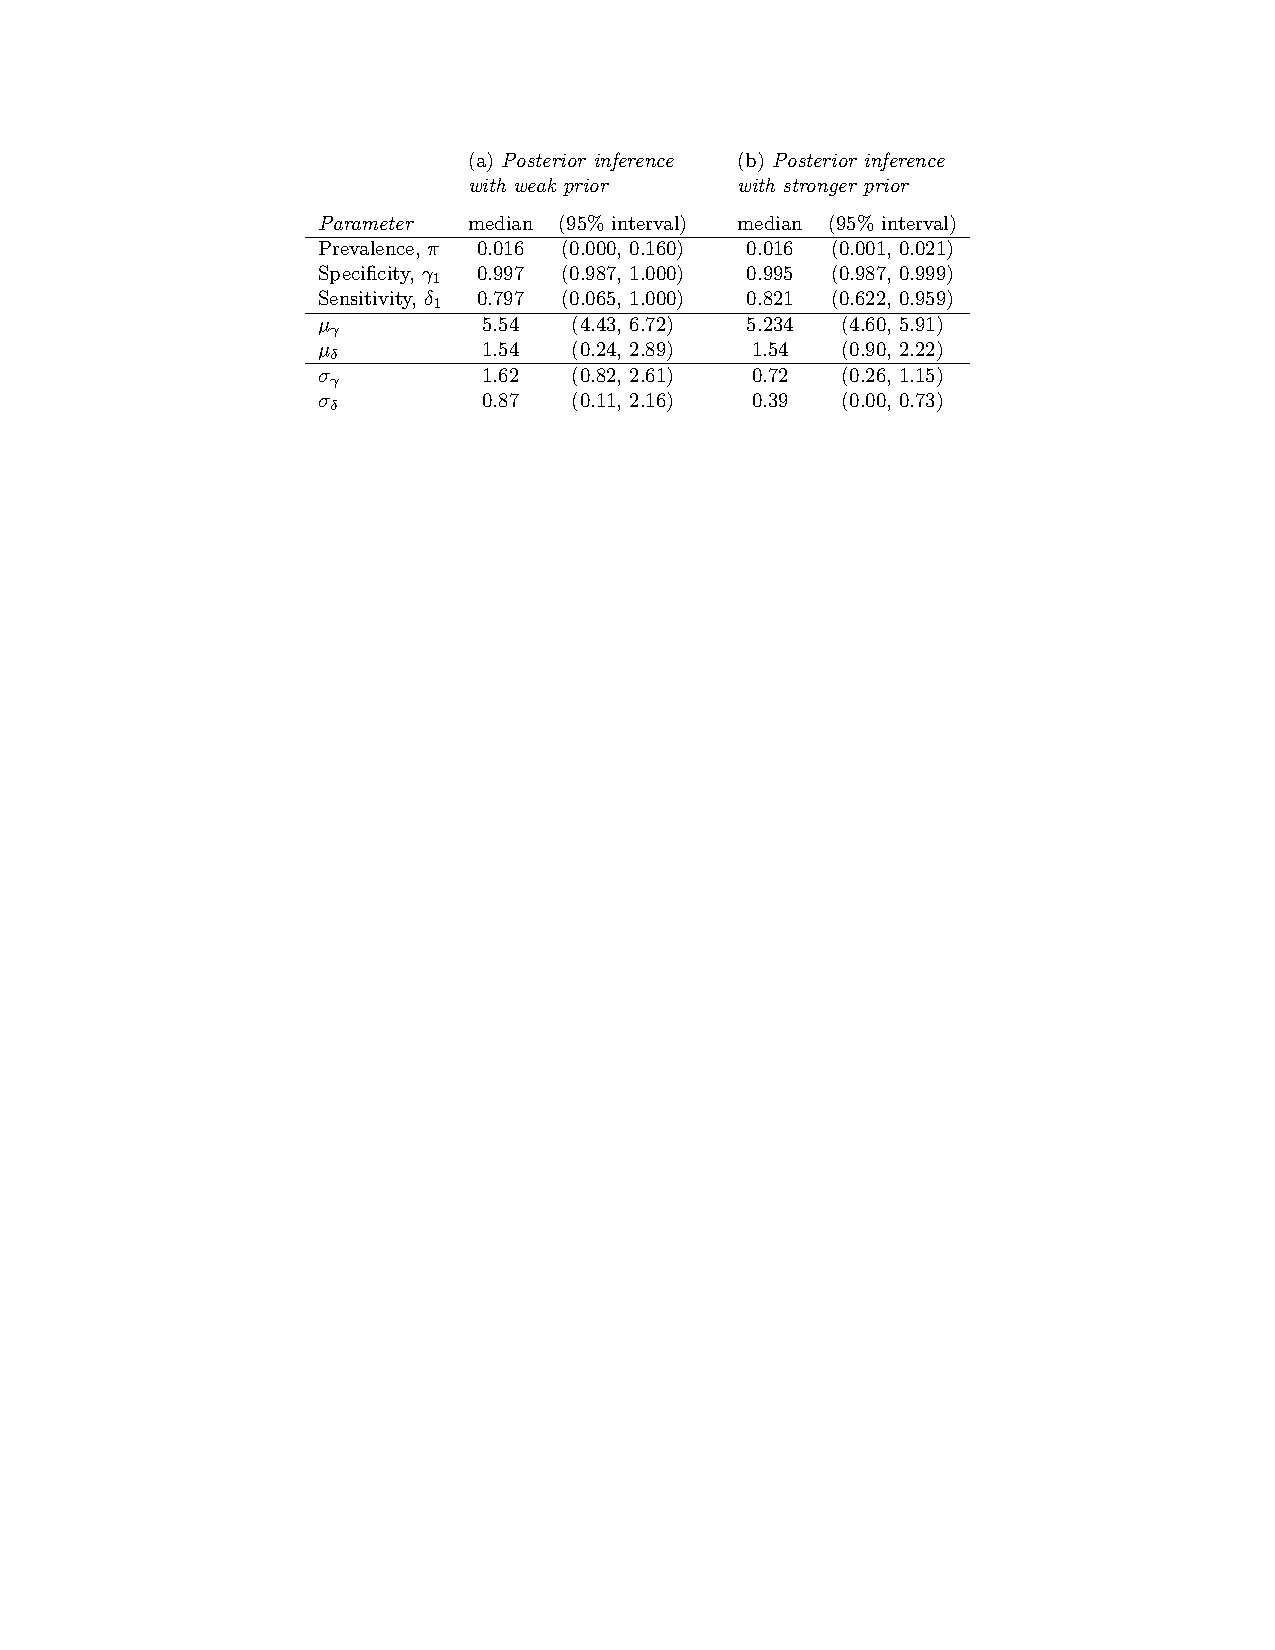
\includegraphics[width=0.9\textwidth]{img/results-table.pdf}
\vfill

\sld{Sensitivity analysis}
\begin{subitemize}
  \item \myemph{sensitivity analysis} varies hyperparameter scales $\tau_0,
    \tau_1$
    \vspace*{-6pt}
  \item \myemph{boxes $\tau_1$}:  sensitivity hyperprior in (0.01, 0.25, 0.5, 0.75, 1)
    \vspace*{-6pt}
  \item \myemph{horizontal axis $\tau_0$}: specificity hyperprior (0--1)
    \vspace*{-6pt}
  \item \myemph{vertical axis $\pi$}:  est.\ median \& central 90\% prevalence
  \end{subitemize}
\quad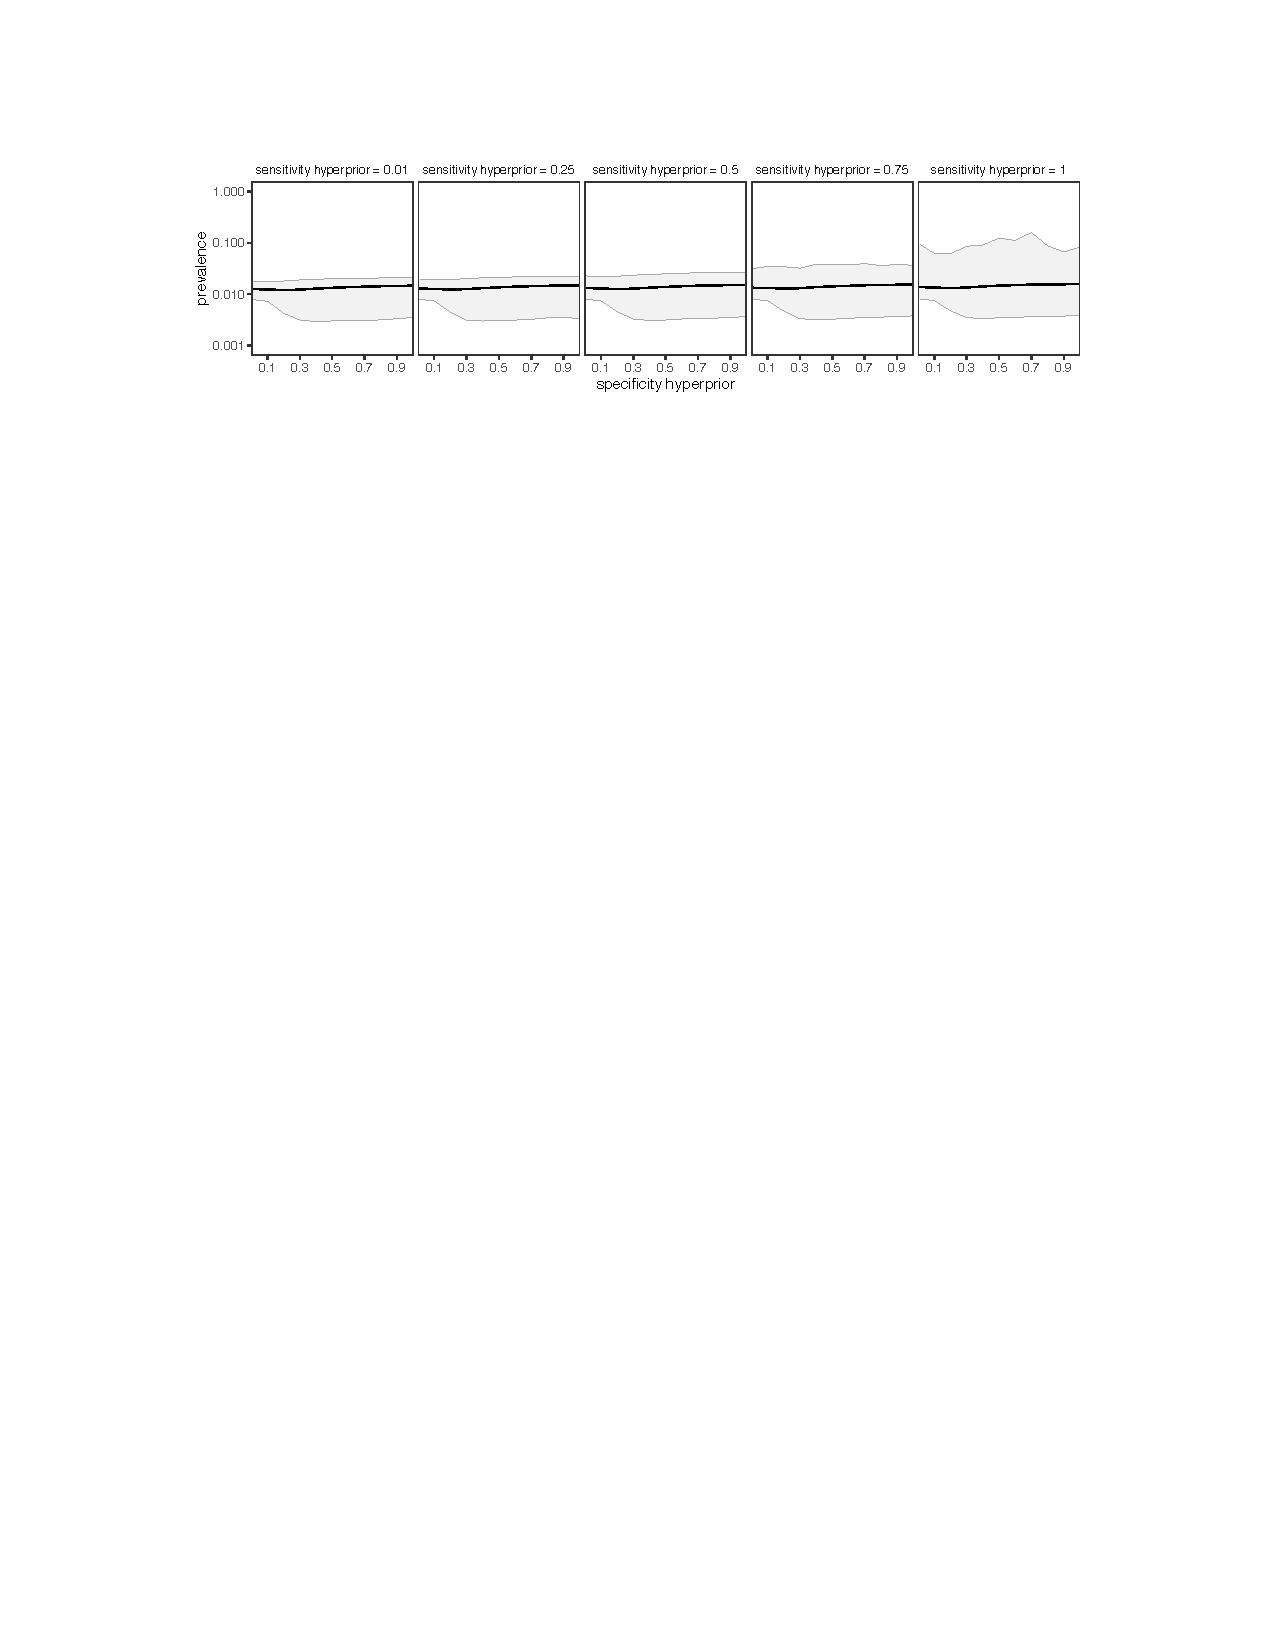
\includegraphics[width=1.05\textwidth]{img/sensitivity-analysis.pdf}    
\begin{subitemize}
  \item prevalence estimate \myemph{not very sensitive} to hyperparameter scale
  \end{subitemize}

\sld{Poststratification}
\begin{itemize}
\item our paper discusses applying \myemph{poststratification} to
  \begin{subitemize}
  \item \myemph{adjust} for differences between \myemph{sample and population}
  \end{subitemize}
\item idea is to let \myemph{prevalence vary} by
  \begin{subitemize}
  \item sex
  \item age
  \item ethnicity 
  \item geolocation plus geolocal predictor (e.g., income)
  \end{subitemize}
\item Bendavid et al. poststratified, but didn't share covariates
\item we poststratified UK (\& Indiana), but no time to present
\end{itemize}

\sld{Implementation}
\begin{itemize}
\item we coded our models in \myemph{Stan}
\item Stan has \myemph{continuous parameters}, so we
  \begin{subitemize}
  \item \myemph{marginalize out} ``missing data'' (disease status
    $z_n$)
  \end{subitemize}
\item \myemph{complete data likelihood}:
  {\small
  \begin{eqnarray*}
    p(y_n, z_n \mid \pi, \theta)
    & = & \textrm{bern}(z_n \mid \pi)
          \\
    & & {} \times \textrm{bern}\big(y_n \mid \textrm{ifelse}(z_n,
        \ \  \theta_{1,
      \, kk[n]},  \ \ 1 - \theta_{0, \, kk[n]})\big)
  \end{eqnarray*}}
  \item \myemph{likelihood}:
  $$\textrm{Pr}\left[y_n = 1 \mid \pi, \theta\right]
    = \underbrace{\pi \cdot \theta_{1, \, kk[n]}}_{\textrm{true
        positive rate}}
    + \underbrace{(1 - \pi) \cdot (1 - \theta_{0, \,
        kk[n]})}_{\textrm{false negative rate}}$$
\end{itemize}
\end{document}

